\documentclass[12pt, a4paper]{article}

% 基礎套件
\usepackage[margin=2.5cm]{geometry}
\usepackage{xeCJK} % 支援中文
\usepackage{graphicx}
\usepackage{listings}
\usepackage{xcolor}
\usepackage{booktabs}
\usepackage{longtable}
\usepackage{hyperref}
\usepackage{float}

% 設定字體
\setCJKmainfont{Microsoft JhengHei}[
    AutoFakeBold=2.5,
    AutoFakeItalic=true
]

% 設定程式碼樣式
\definecolor{codegreen}{rgb}{0,0.6,0}
\definecolor{codegray}{rgb}{0.5,0.5,0.5}
\definecolor{codepurple}{rgb}{0.58,0,0.82}
\definecolor{backcolour}{rgb}{0.95,0.95,0.92}

\lstset{
    language=VHDL,
    backgroundcolor=\color{backcolour},   
    commentstyle=\color{codegreen},
    keywordstyle=\color{magenta},
    numberstyle=\tiny\color{codegray},
    stringstyle=\color{codepurple},
    basicstyle=\ttfamily\small,
    breakatwhitespace=false,         
    breaklines=true,                 
    captionpos=b,                    
    keepspaces=true,                 
    numbers=left,                    
    numbersep=5pt,                  
    showspaces=false,                
    showstringspaces=false,
    showtabs=false,                  
    tabsize=2,
    frame=single
}

\title{微處理器系統實驗報告 - Lab 05 \\ \Large N位元左/右移位萬用暫存器設計}
\author{第 19 組 \\ 資工二 \\ 113590051 楊承諭、113590017 黃楷程}
\date{2026年5月13日}

\begin{document}

\maketitle
\newpage

\section{實驗目的}
\begin{enumerate}
    \item \textbf{學習使用 VHDL 的 GENERIC 關鍵字}：建立具備可變位元長度的硬體模組，提高程式碼的重用性。
    \item \textbf{掌握 PROCESS 區塊內的 FOR LOOP 語法}：透過迴圈結構簡潔地實作資料位移邏輯。
    \item \textbf{實作並驗證萬用暫存器}：整合同步清除 (Clear)、平行載入 (Parallel Load) 與左/右移位功能。
\end{enumerate}

\section{實驗原理與邏輯設計}
本實驗設計一個 N 位元（在此實作為 10 位元）的同步電路，其行為受時脈 \texttt{clk} 正緣觸發。控制訊號優先權如下：

\begin{enumerate}
    \item \textbf{同步清除 (clean='1')}：在時脈正緣觸發時，將暫存器歸零。
    \item \textbf{平行載入 (load='1')}：將 10 位元輸入端 \texttt{di} 的數值直接載入。
    \item \textbf{左移 (lr\_sel='1')}：內容向 MSB 移動，LSB 補入 \texttt{sdi}。
    \item \textbf{右移 (lr\_sel='0')}：內容向 LSB 移動，MSB 補入 \texttt{sdi}。
\end{enumerate}

\section{實驗步驟與程式碼實作}

\subsection{VHDL 核心邏輯}
本實驗採用行為級描述，利用 \texttt{FOR LOOP} 處理位元移動。

\begin{lstlisting}[language=VHDL, caption=N\_bit\_DFF.vhd 核心移位邏輯]
-- 左移邏輯範例
for i in N-1 downto 1 loop
    reg(i) <= reg(i-1);
end loop;
reg(0) <= sdi;

-- 右移邏輯範例
for i in 0 to N-2 loop
    reg(i) <= reg(i+1);
end loop;
reg(N-1) <= sdi;
\end{lstlisting}

\subsection{硬體腳位配置 (Pin Assignment)}
\begin{table}[H]
\centering
\begin{tabular}{@{}lll@{}}
\toprule
訊號名稱 & 功能說明 & FPGA 腳位 (Cyclone IV E) \\
\midrule
\texttt{clk} & 時脈輸入 & PIN\_M23 (KEY0) \\
\texttt{clean} & 同步清除 & PIN\_AB23 (SW12) \\
\texttt{load} & 平行載入 & PIN\_AC24 (SW10) \\
\texttt{lr\_sel} & 移位方向 & PIN\_AB24 (SW11) \\
\texttt{sdi} & 串列輸入 & PIN\_AA24 (SW13) \\
\texttt{di[9..0]} & 10位元平行輸入 & PIN\_AB25 $\sim$ PIN\_AB28 \\
\texttt{qo[9..0]} & 10位元輸出 (LED) & PIN\_G17 $\sim$ PIN\_G19 \\
\bottomrule
\end{tabular}
\end{table}

\section{實驗結果與驗證}

\subsection{實作照片紀錄}
\begin{longtable}{p{6cm} c}
\toprule
狀態描述 & 實體照片 \\
\midrule
\textbf{同步清除}：開啟清除開關並按壓時脈，LED 全滅。 & 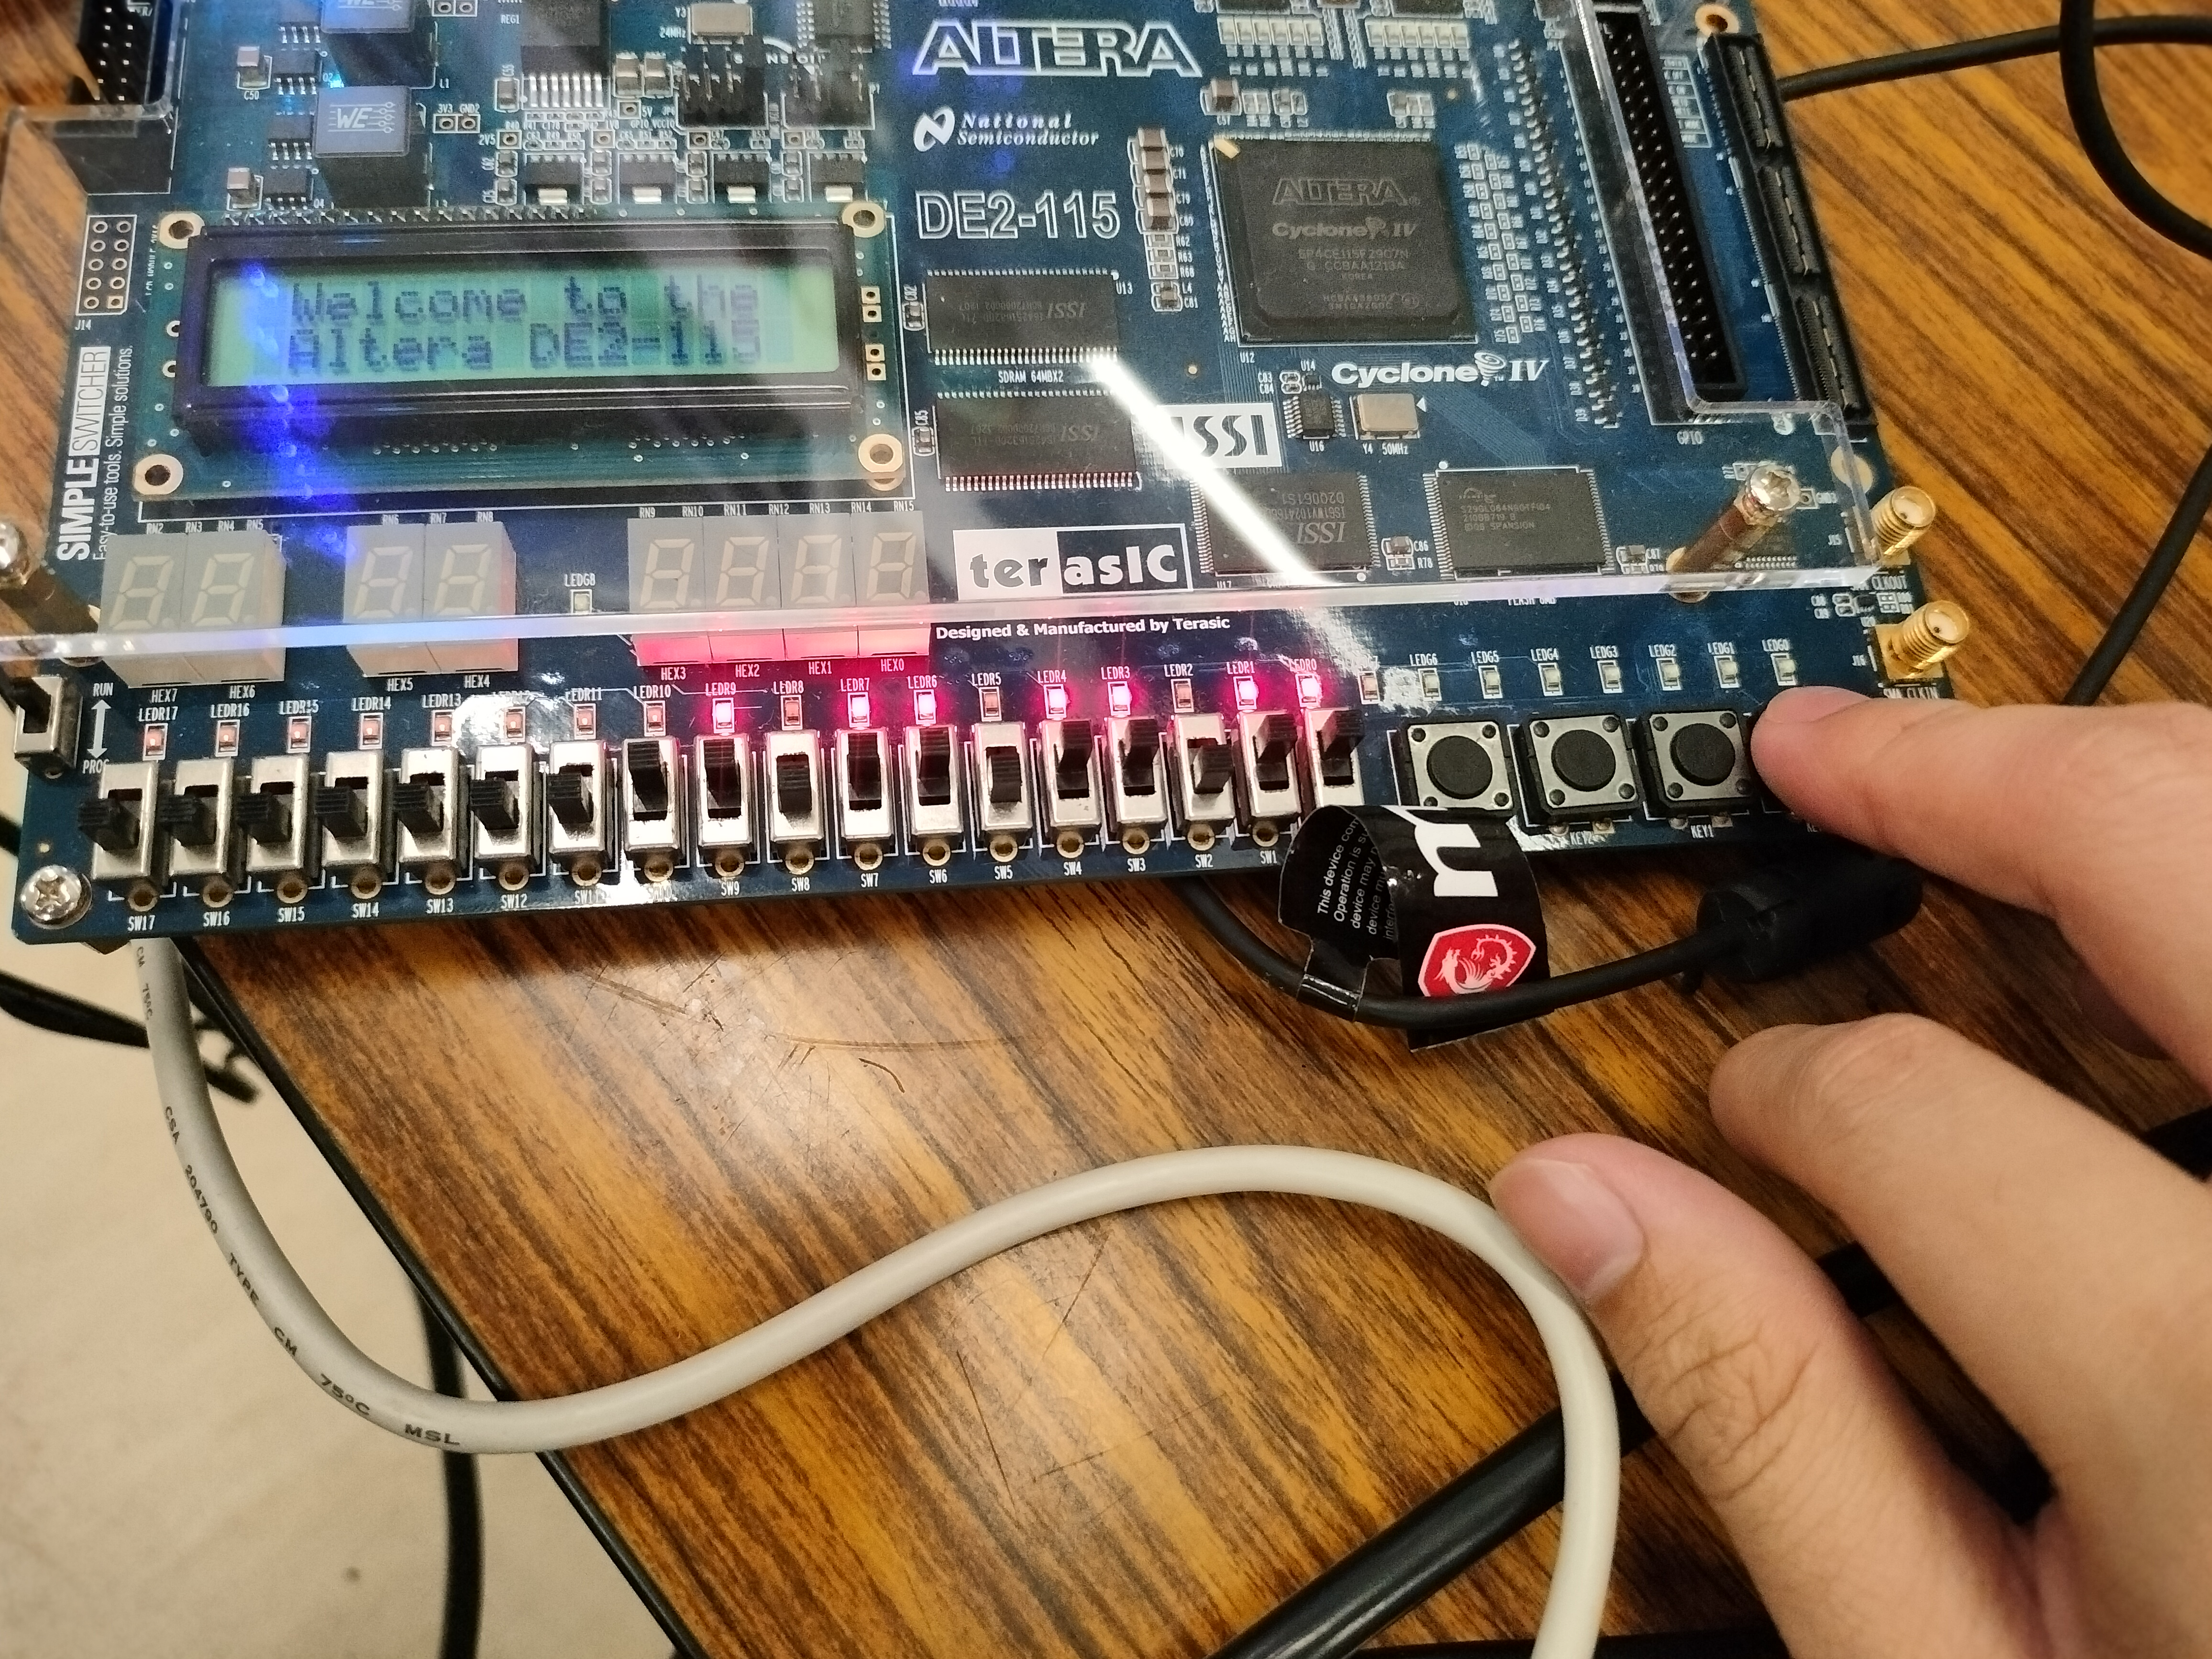
\includegraphics[width=0.45\textwidth]{./Photo/IMG20260513212848.jpg} \\
\textbf{平行載入}：載入開關設定之數值。 & 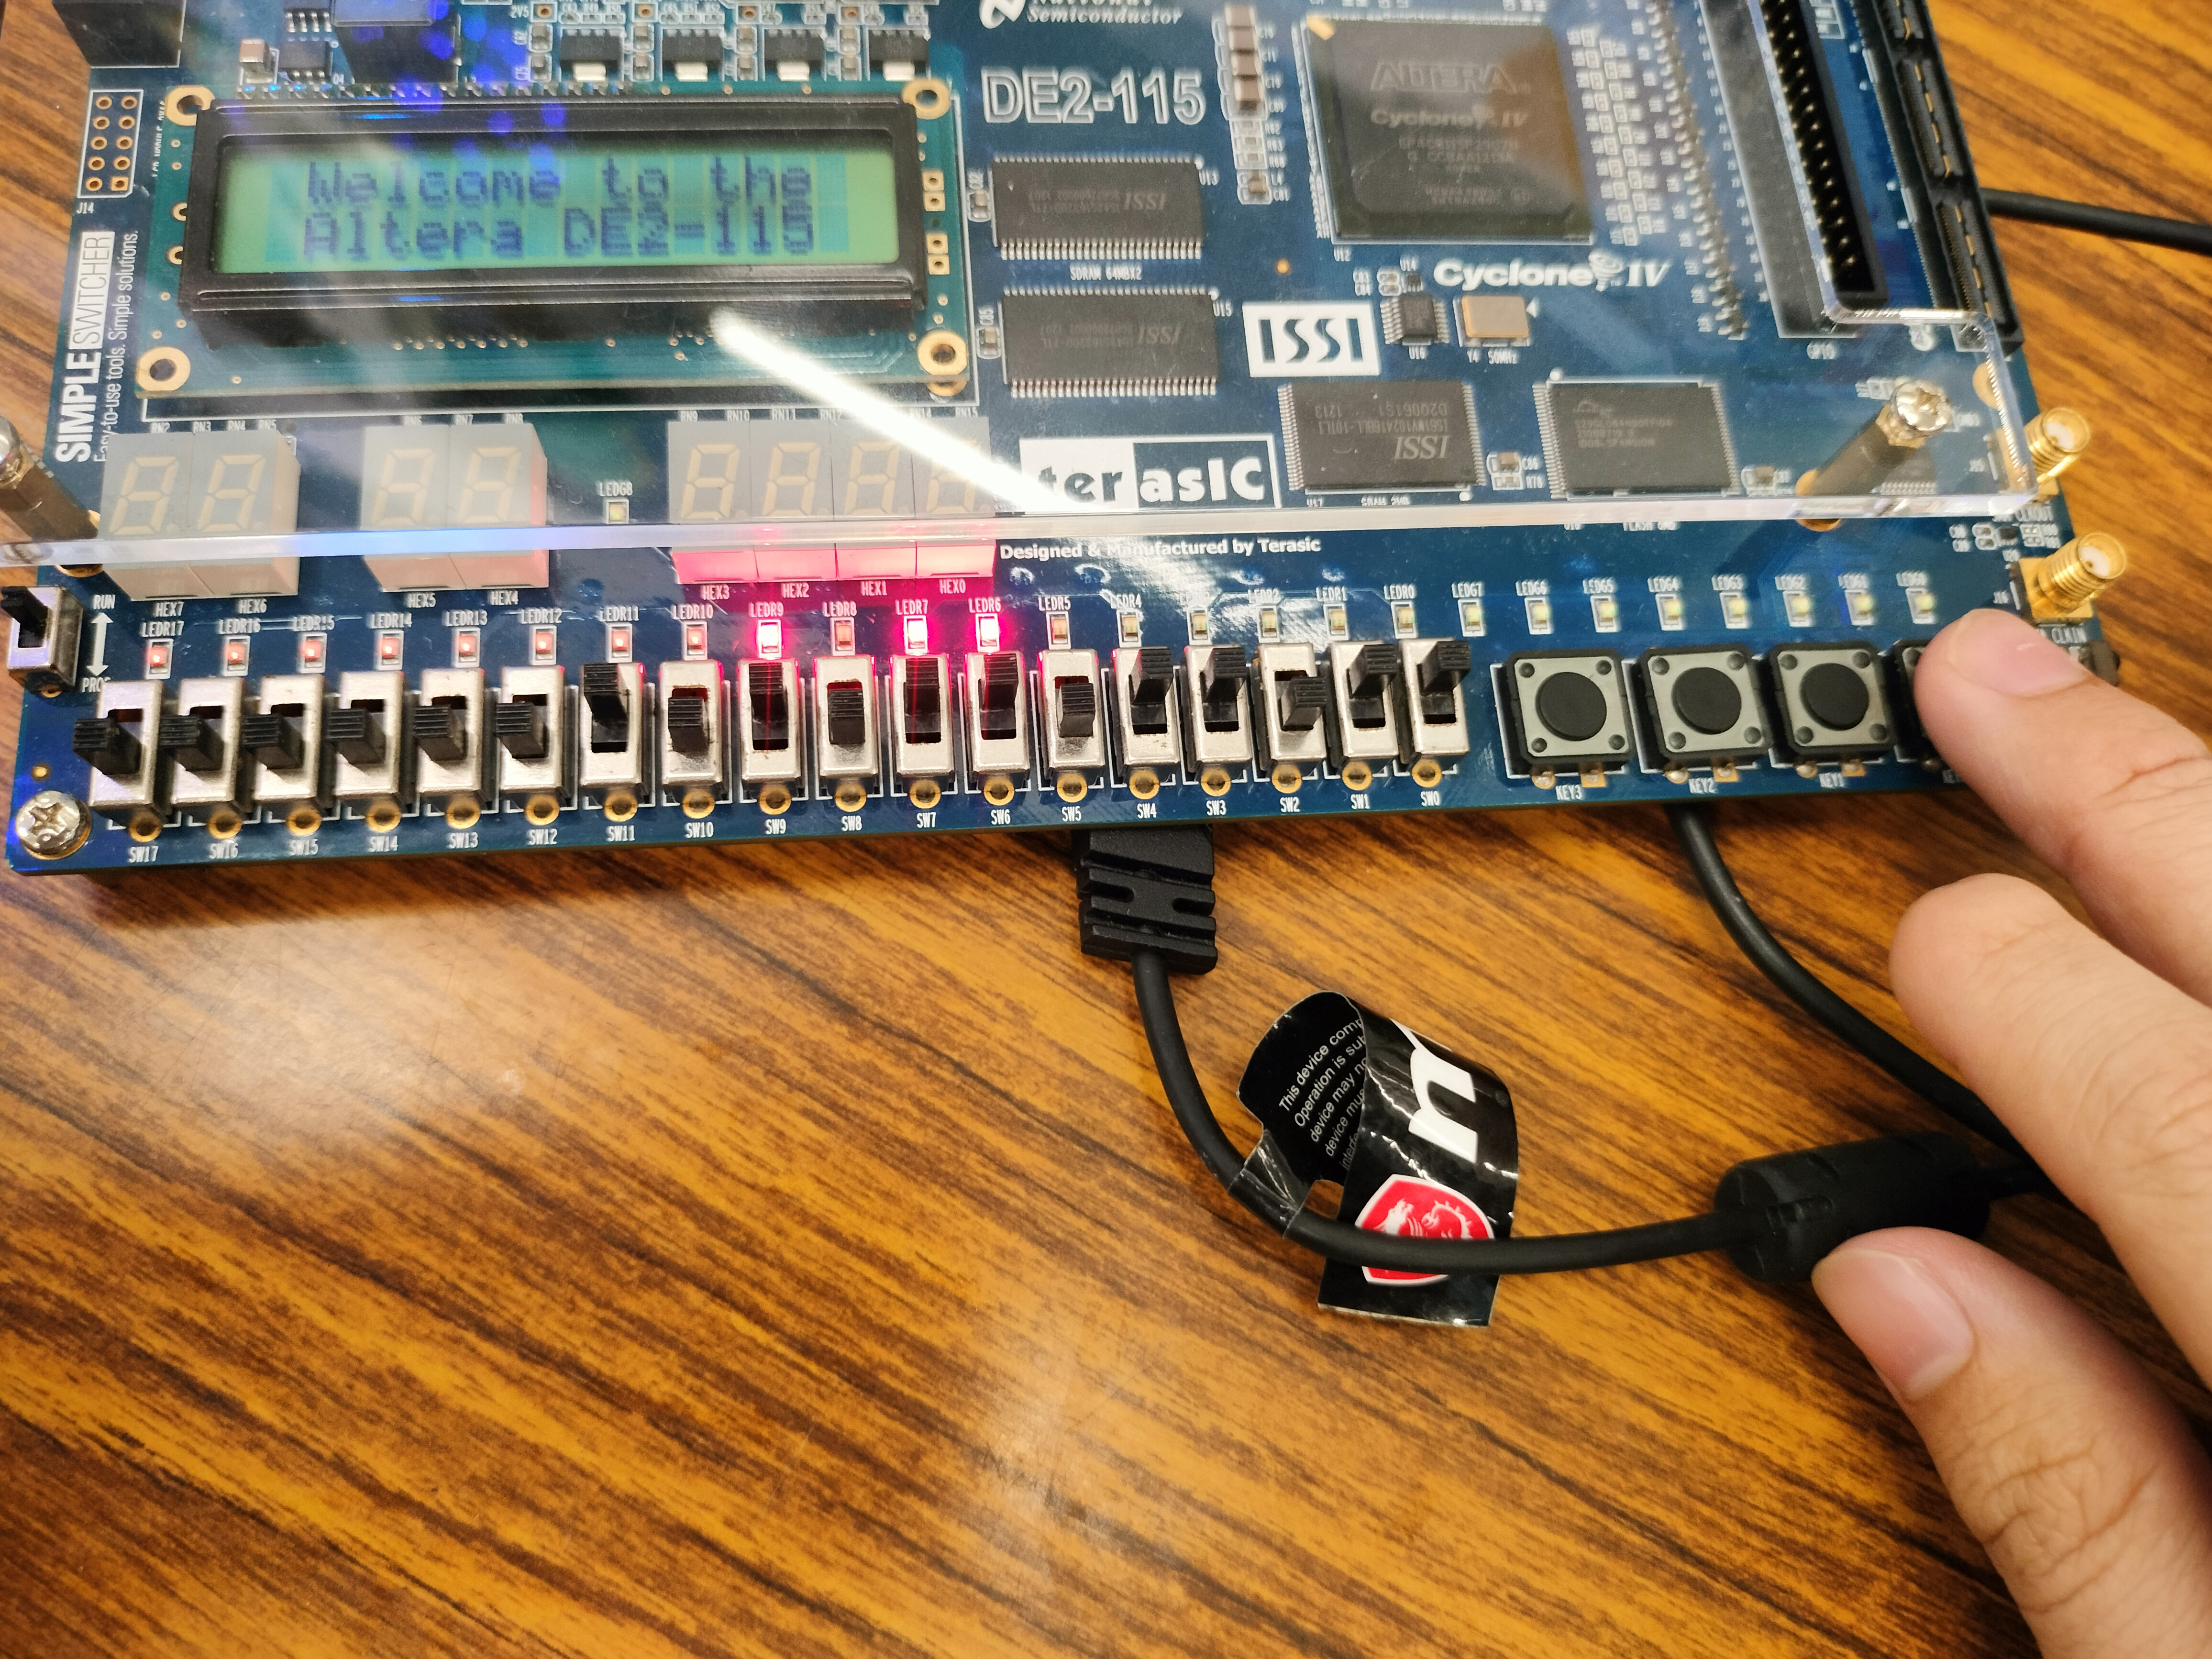
\includegraphics[width=0.45\textwidth]{./Photo/IMG20260513213439.jpg} \\
\textbf{左移過程}：觀察位元逐位向左移動。 & 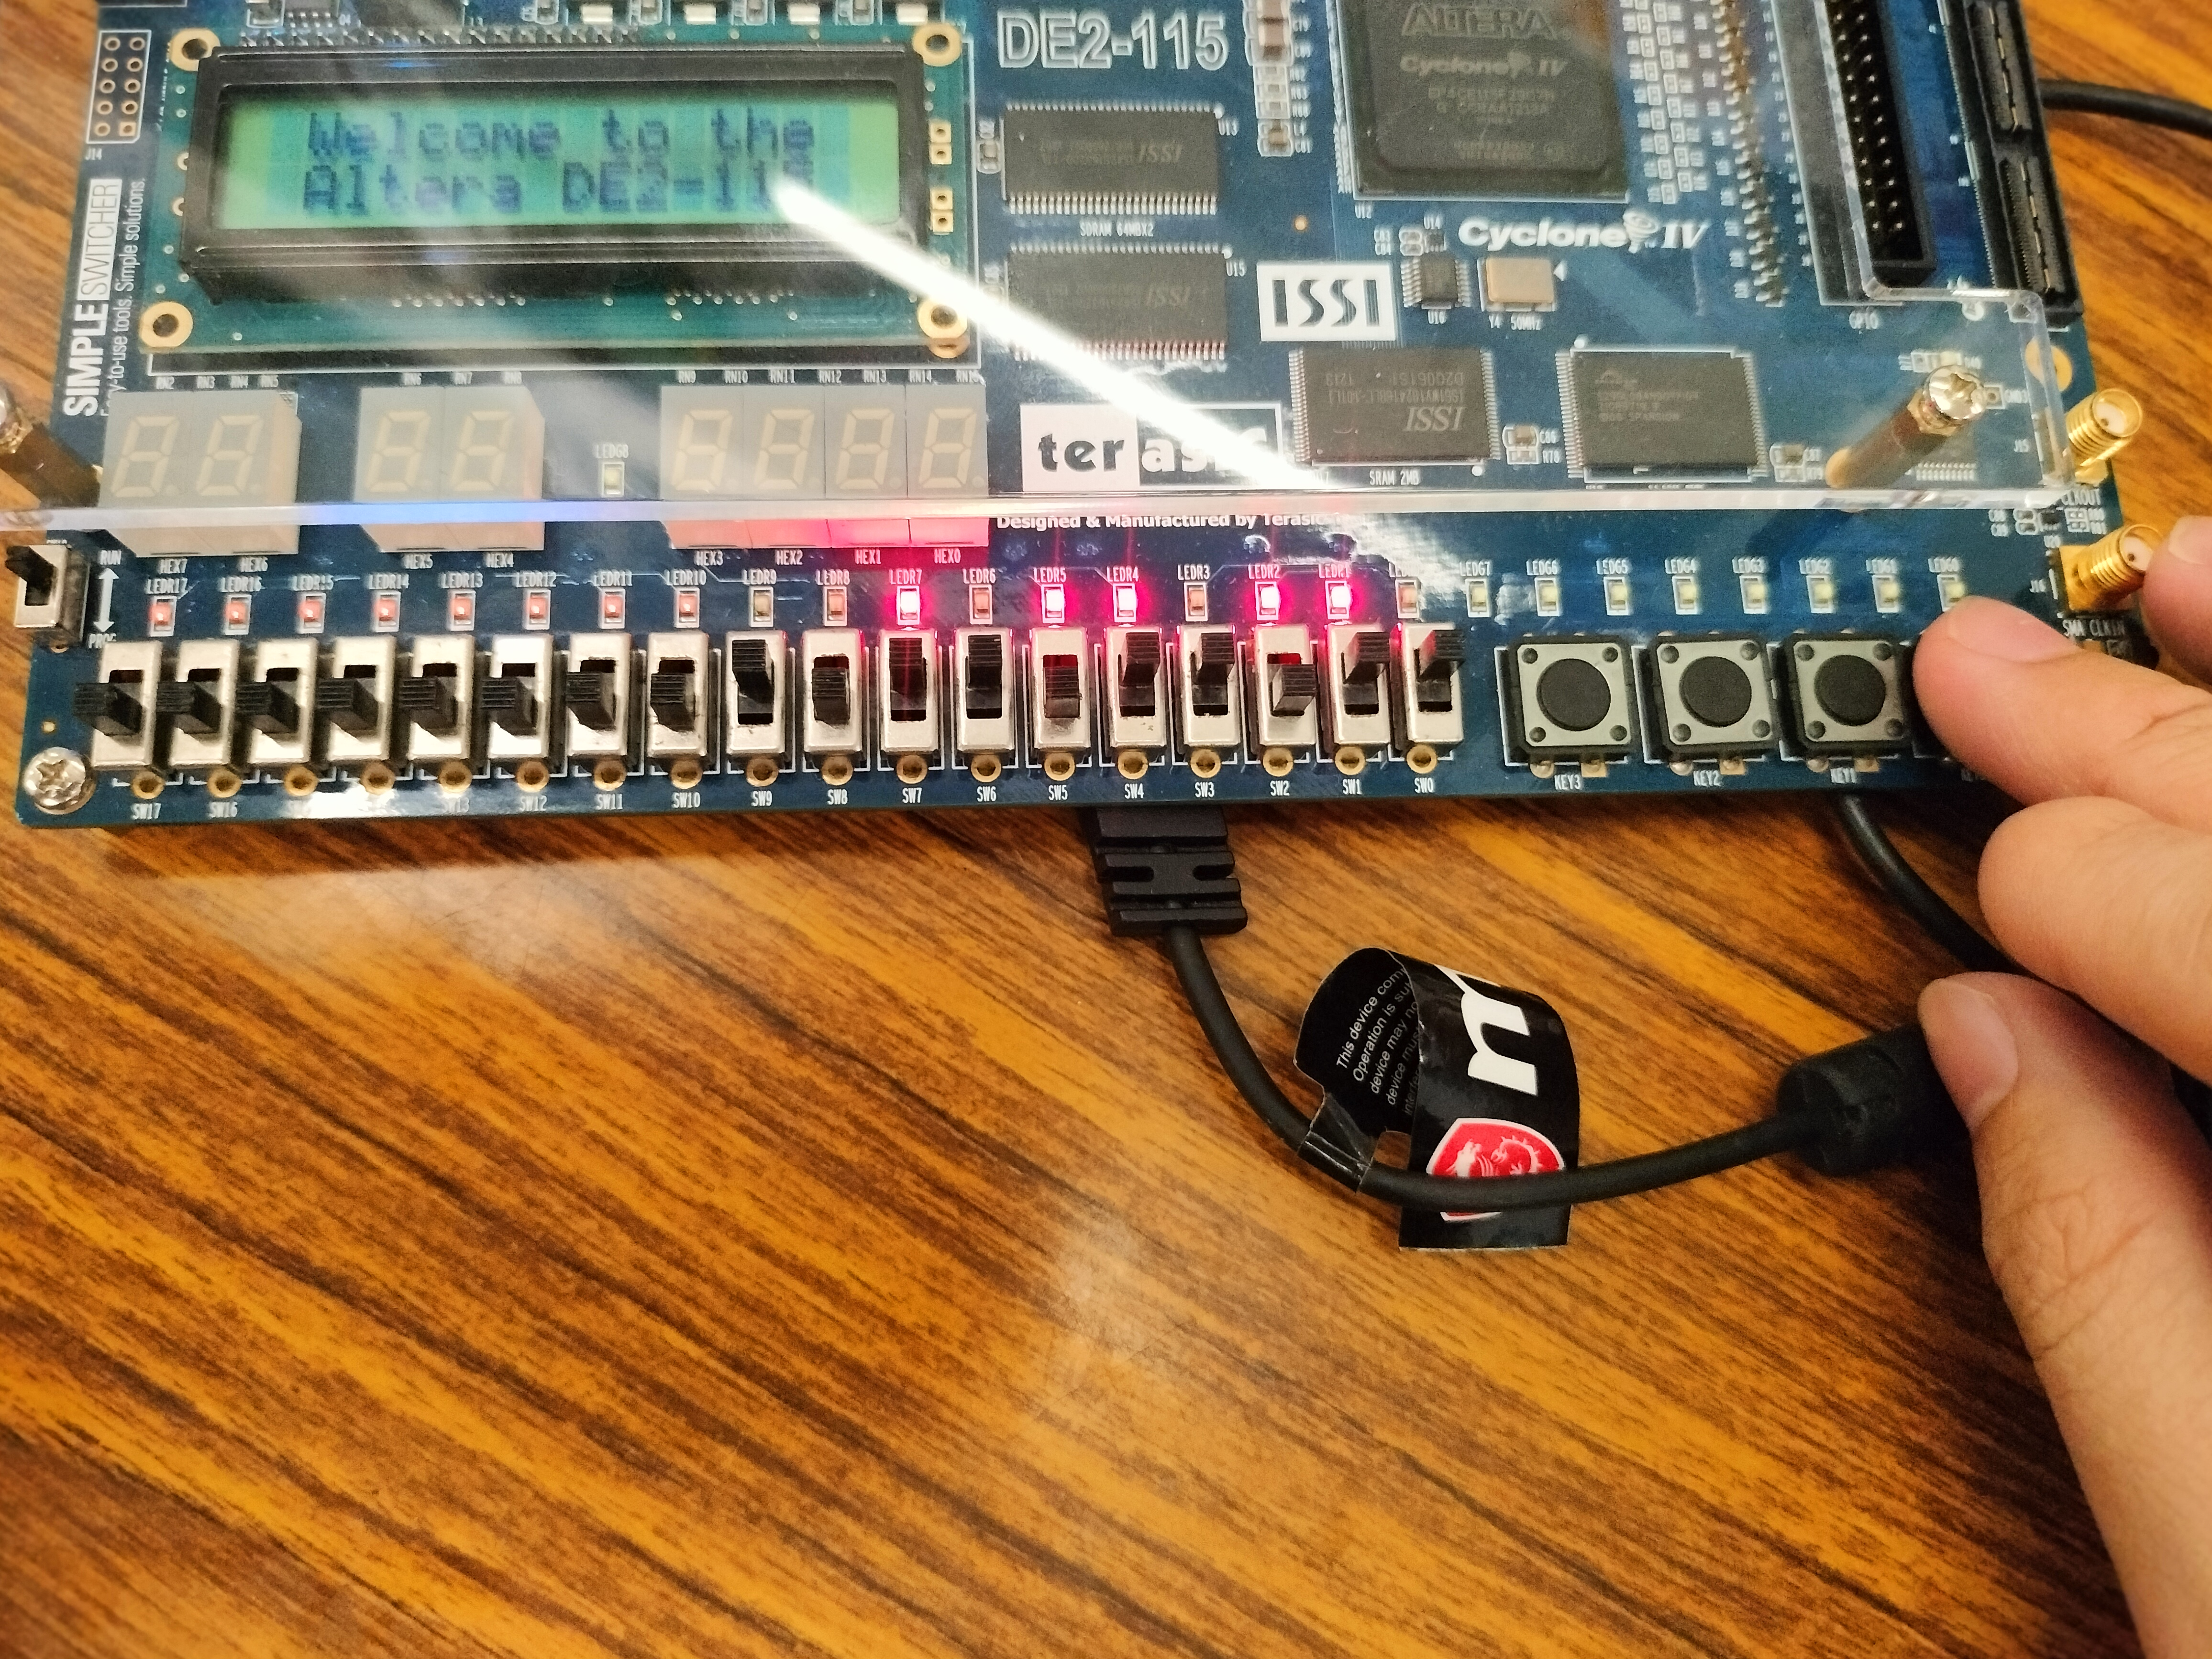
\includegraphics[width=0.45\textwidth]{./Photo/IMG20260513213633.jpg} \\
\textbf{串列輸入 (SDI)}：驗證新位元補入。 & 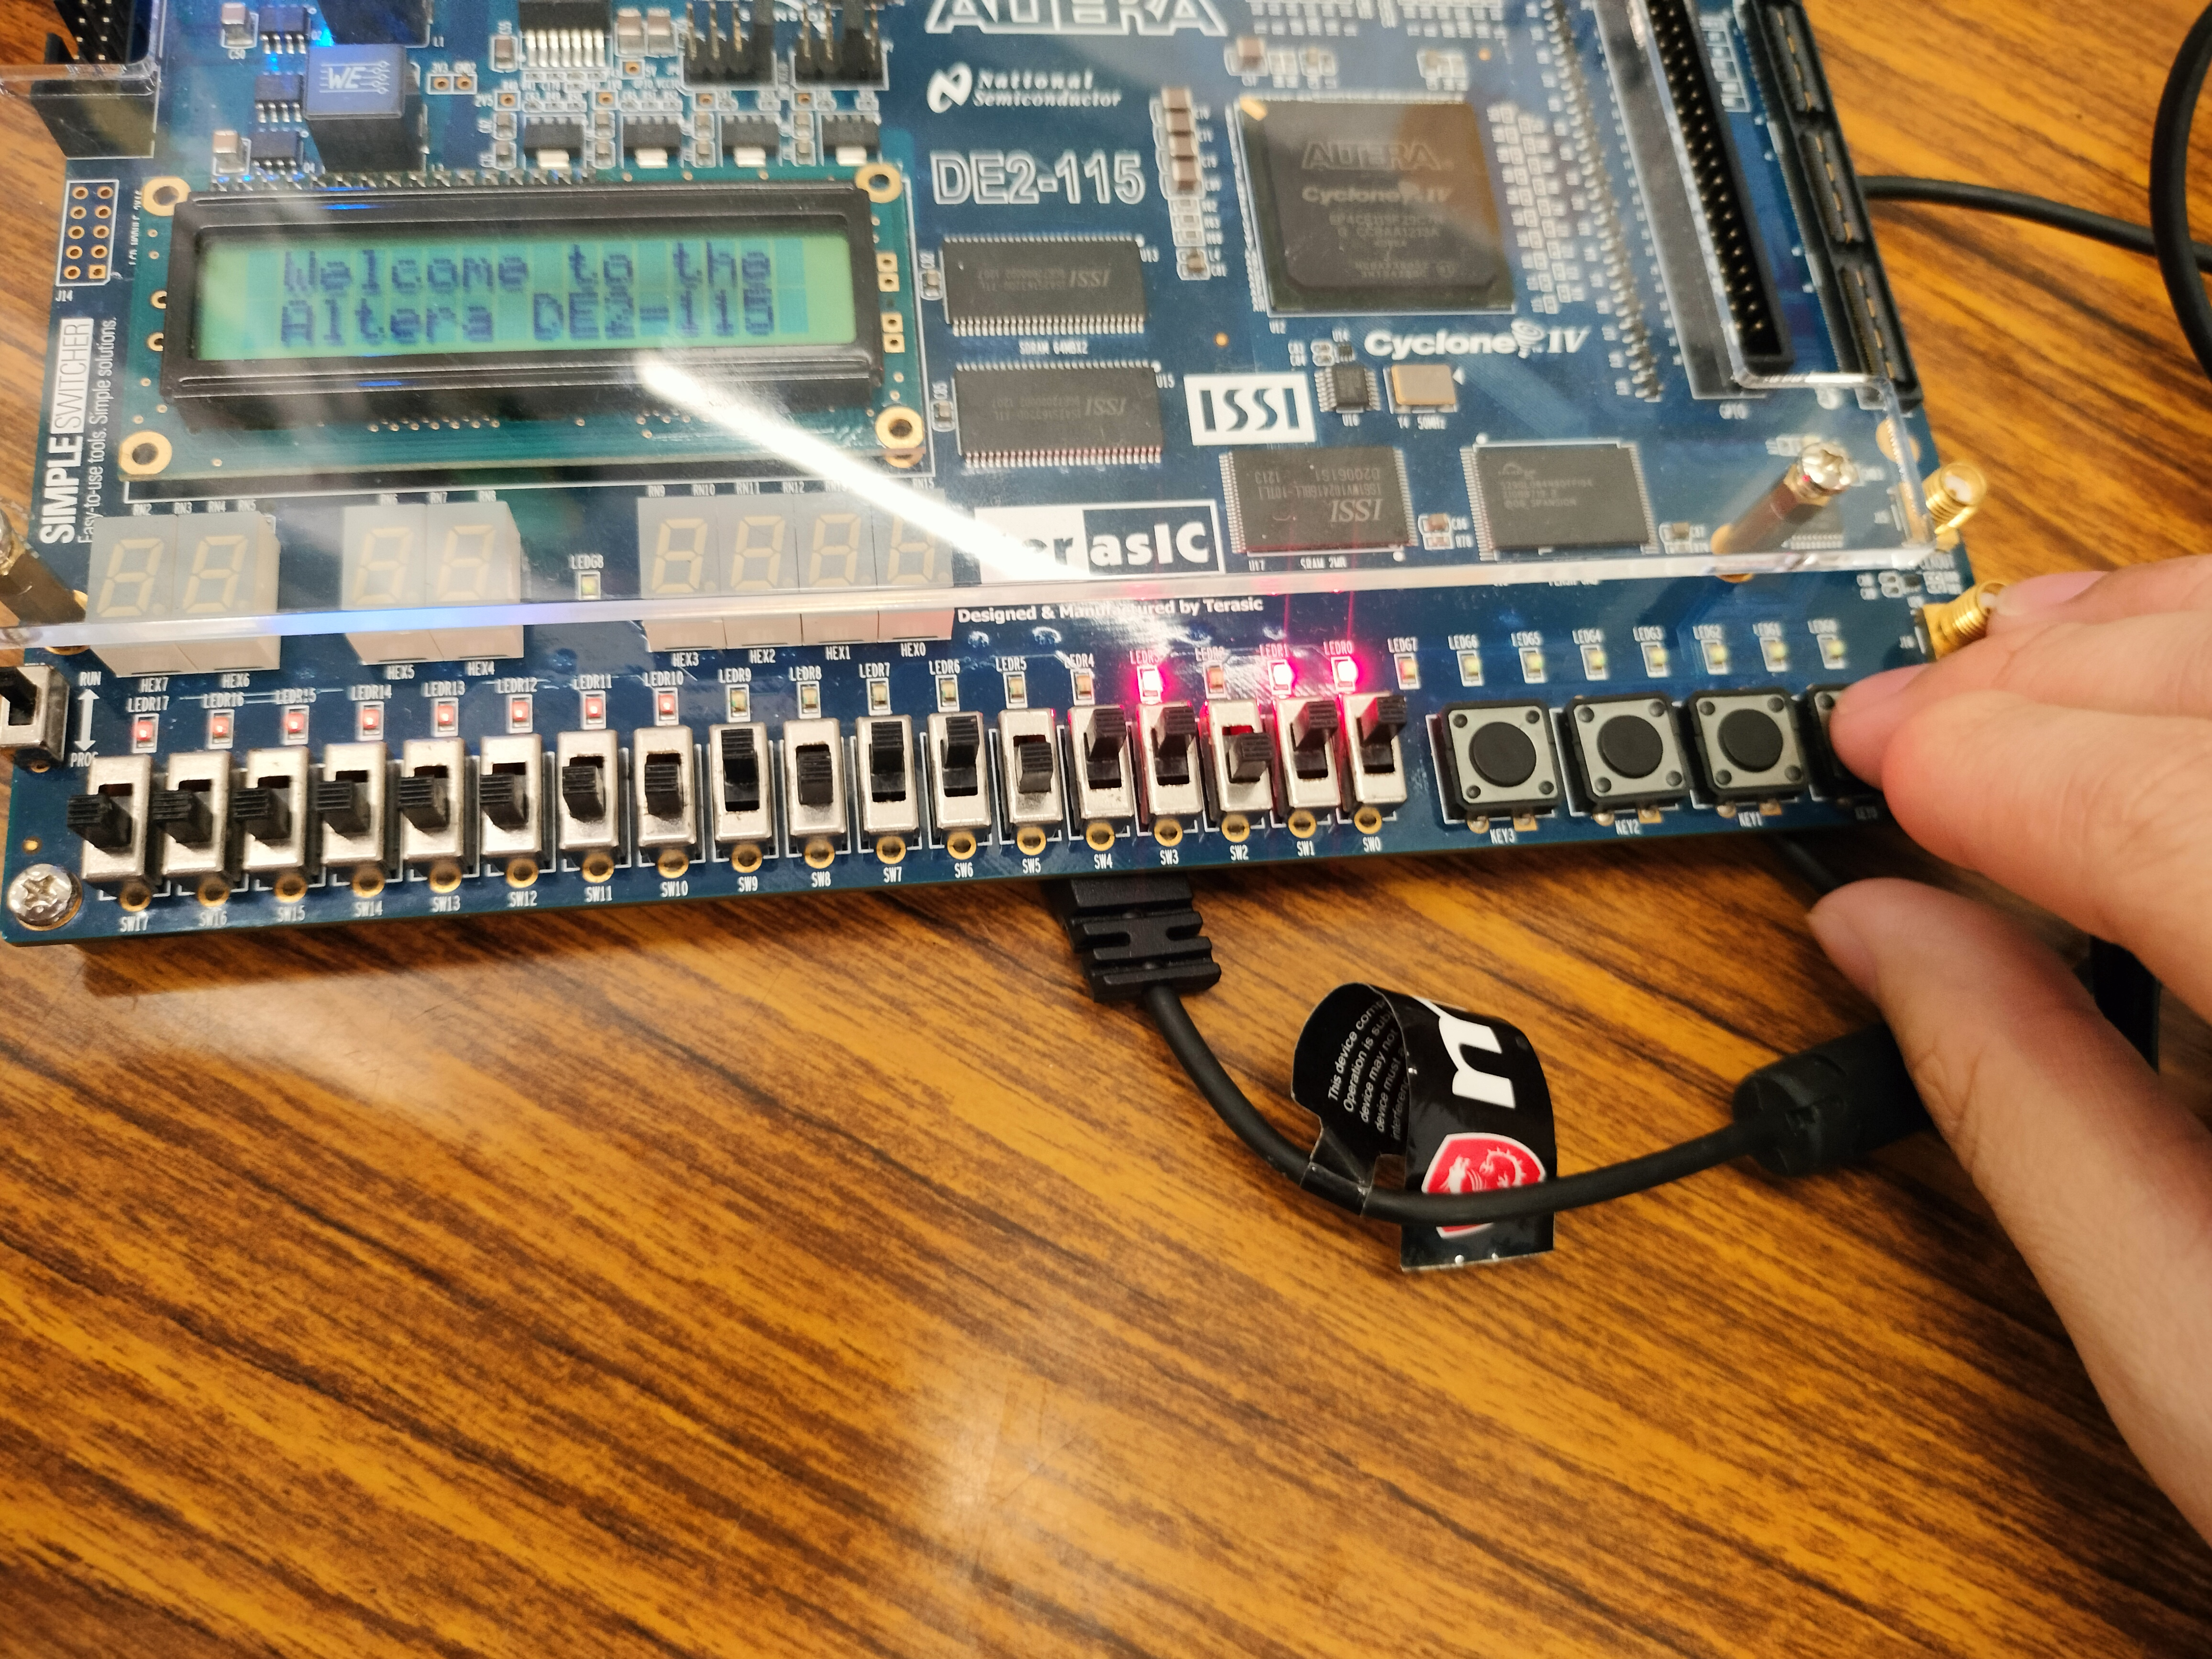
\includegraphics[width=0.45\textwidth]{./Photo/IMG20260513213719.jpg} \\
\textbf{右移操作}：切換方向後位元向右移動。 & 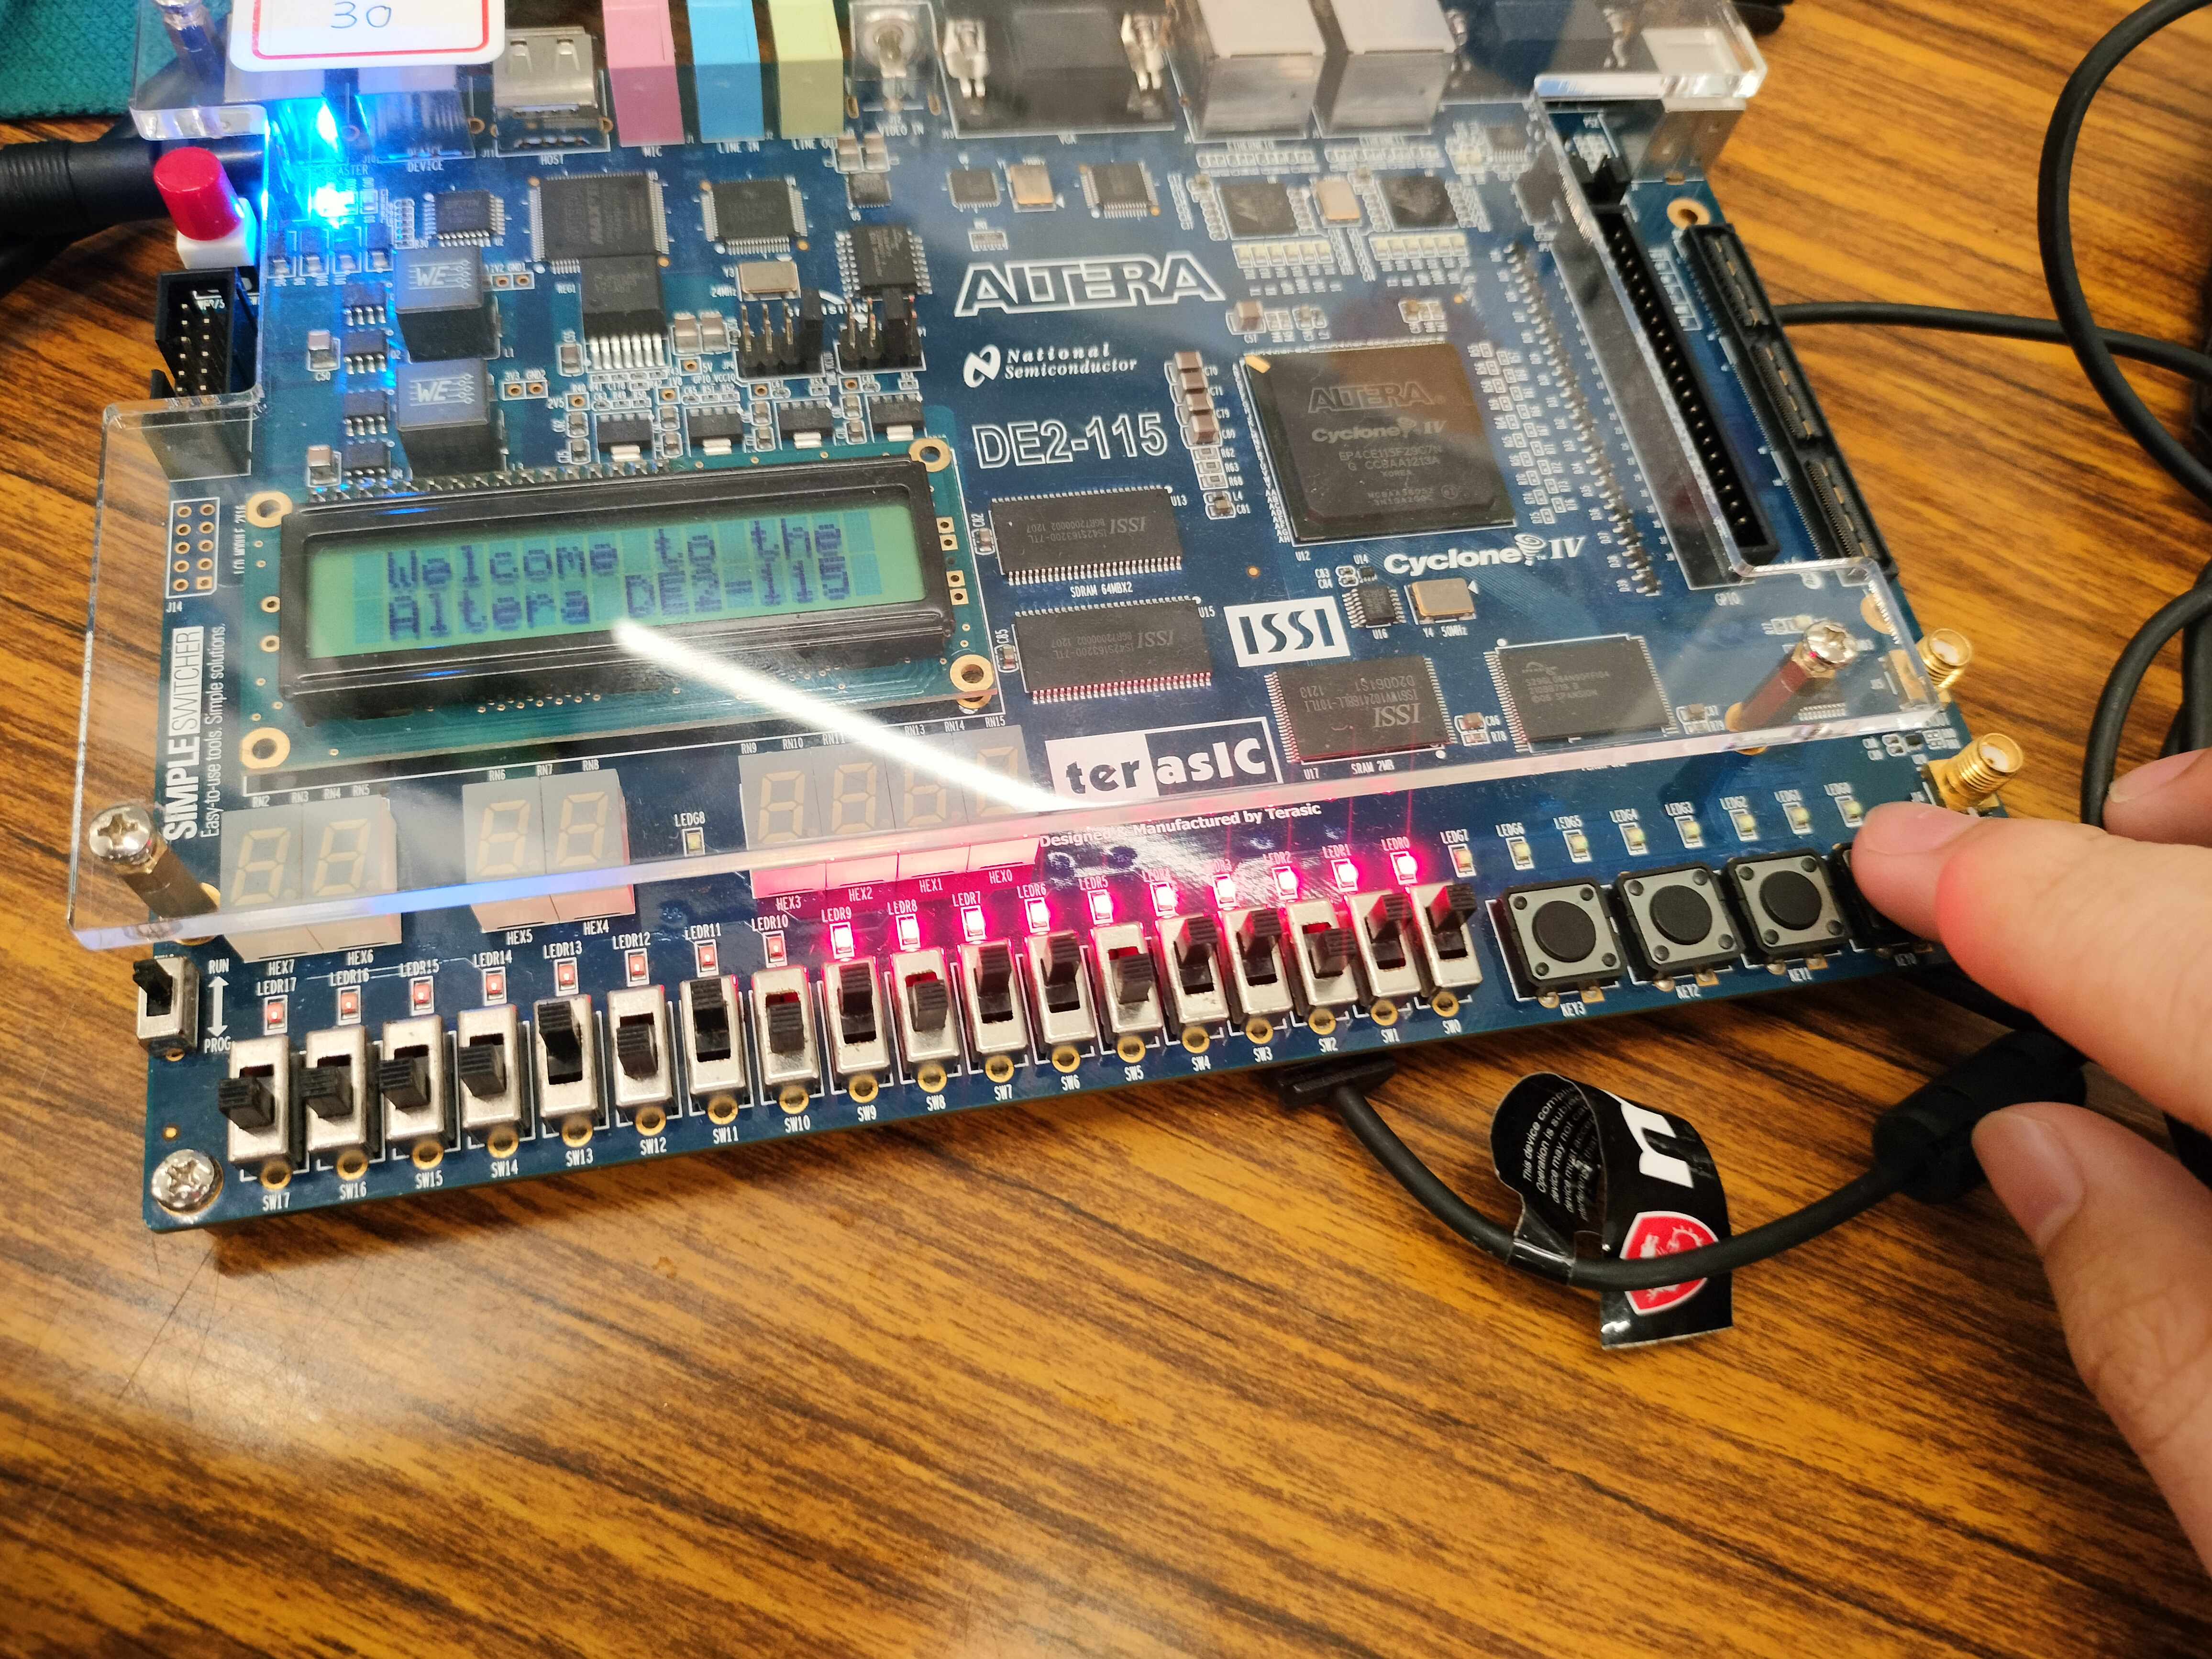
\includegraphics[width=0.45\textwidth]{./Photo/IMG20260513214908.jpg} \\
\bottomrule
\end{longtable}

\section{結論與心得}
透過本實驗，我們深刻理解了 \texttt{GENERIC} 在硬體描述語言中的彈性，以及 \texttt{FOR LOOP} 如何在合成時轉化為平行硬體結構。同步邏輯的設計確保了訊號在時脈緣觸發下的穩定性。

\section{組員貢獻比例}
\begin{table}[H]
\centering
\begin{tabular}{@{}llll@{}}
\toprule
姓名 & 學號 & 貢獻比例 & 負責內容 \\
\midrule
楊承諭 & 113590051 & 75\% & 程式開發、硬體測試 \\
黃楷程 & 113590017 & 25\% & 報告撰寫 \\
\bottomrule
\end{tabular}
\end{table}

\end{document}
